\documentclass[10pt]{elsarticle}

  \usepackage{pgfplots}
\pgfplotsset{compat=newest}
%% the following commands are needed for some matlab2tikz features
\usetikzlibrary{plotmarks}
\usetikzlibrary{arrows.meta}
\usepgfplotslibrary{patchplots}
\usepackage{grffile}
\usepackage{amsmath}
\usepackage{lineno}


%\usepackage{fullpage}
\usepackage[top=1in, bottom=1in, left=0.8in, right=1in]{geometry}
\usepackage{multicol}
\usepackage{caption}
\usepackage{subcaption}
\usepackage{hyperref}
\usepackage{xcolor}
\usepackage{graphicx,psfrag}
\usepackage[pdf]{pstricks}

\definecolor{lightblue}{rgb}{.80,.9,1}
\newcommand{\hl}[1]
    {\par\colorbox{lightblue}{\parbox{\linewidth}{#1}}}

\newcommand{\defn}{\stackrel{\textrm{\scriptsize def}}{=}}

\setlength{\columnsep}{0.1pc}

\title{Numerical Scheme for the Generalised Serre-Green-Naghdi Model}
%\author{Christopher Zoppou -- \texttt{christopher.zoppou@anu.edu.au}, Dimitrios Mitsotakis -- \texttt{dmitsot@gmail.com}, Stephen Roberts -- \texttt{stephen.roberts@anu.edu.au}, Jordan Pitt}

% TIME ON EVERY PAGE AS WELL AS THE FILE NAME
\usepackage{fancyhdr}
\usepackage{currfile}
\usepackage[us,12hr]{datetime} % `us' makes \today behave as usual in TeX/LaTeX
\fancypagestyle{plain}{
\fancyhf{}
\rfoot{\emph{\footnotesize \textcopyright  Serre Notes by C. Zoppou, D. Mitsatakis and S. Roberts.}
 \\ File Name: {\currfilename} \\ Date: {\ddmmyyyydate\today} at \currenttime}
\lfoot{Page \thepage}
\renewcommand{\headrulewidth}{0pt}}
\pagestyle{plain}

\definecolor{mycolor1}{rgb}{0.00000,0.44700,0.74100}%
\definecolor{mycolor2}{rgb}{0.85000,0.32500,0.09800}%
\definecolor{mycolor3}{rgb}{0.92900,0.69400,0.12500}%
\definecolor{mycolor4}{rgb}{0.49400,0.18400,0.55600}%
\definecolor{mycolor5}{rgb}{0.46600,0.67400,0.18800}% 
\definecolor{mycolor6}{rgb}{0.30100,0.74500,0.93300}%
\definecolor{mycolor7}{rgb}{0.63500,0.07800,0.18400}%

\newcommand\T{\rule{0pt}{3ex }}       % Top table strut
\newcommand\B{\rule[-4ex]{0pt}{4ex }} % Bottom table strut

\newcommand\TM{\rule{0pt}{2.8ex }}       % Top matrix strut
\newcommand\BM{\rule[-2ex]{0pt}{2ex }} % Bottom matrix strut

\newcommand{\vecn}[1]{\boldsymbol{#1}}
\DeclareRobustCommand{\solidrule}[1][0.25cm]{\rule[0.5ex]{#1}{1.5pt}}

\DeclareRobustCommand{\dashedrule}{\mbox{%
		\solidrule[2mm]\hspace{2mm}\solidrule[2mm]}}

\DeclareRobustCommand{\tikzcircle}[1]{\tikz{\filldraw[#1] (0,0) circle (0.5ex);}}	
	
	
\DeclareRobustCommand{\squaret}[1]{\tikz{\draw[#1,thick] (0,0) rectangle (0.2cm,0.2cm);}}
\DeclareRobustCommand{\circlet}[1]{\tikz{\draw[#1,thick] (0,0) circle [radius=0.1cm];}}
\DeclareRobustCommand{\trianglet}[1]{\tikz{\draw[#1,thick] (0,0) --
		(0.25cm,0) -- (0.125cm,0.25cm) -- (0,0);}}
\DeclareRobustCommand{\crosst}[1]{\tikz{\draw[#1,thick] (0cm,0cm) --
		(0.1cm,0.1cm) -- (0cm,0.2cm) -- (0.1cm,0.1cm) -- (0.2cm,0.2cm) -- (0.1cm,0.1cm)-- (0.2cm,0cm);}}
\DeclareRobustCommand{\diamondt}[1]{\tikz{\draw[#1,thick] (0,0) --(0.1cm,0.15cm) -- (0.2cm,0cm) -- (0.1cm,-0.15cm) -- (0,0)  ;}}
\DeclareRobustCommand{\squareF}[1]{\tikz{\filldraw[#1,fill opacity= 0.3] (0,0) rectangle (0.2cm,0.2cm);}}

\begin{document}

\maketitle

\vspace{-0.3in}
\noindent
\rule{\linewidth}{0.4pt}

\tableofcontents

%-------------------------------------------------
\section{Abstract}
%-------------------------------------------------

Papers Primary focus - to extend the approach outlined in Zoppou,Hank to the gSGN equations. This achieves the following goals:
\begin{itemize}
	\item Extension of numerical scheme (elliptic + conservation solvers) of previous papers for SGN to gSGN
	\item Straightforward 2nd order implementation - demonstrating the use of this method
	\item Validation of the example implementation using analytic solutions for SWWE and SGN (dam-break and soliton) and forced solutions for more general members (only showing a select few)
	\item Method is promising : can handle discontinuities, maintain order of accuracy. However, there are additional challenges (weak disconinuities) and limiting of derivative which will be investigated in another paper. 
\end{itemize}



%-------------------------------------------------
\section{Introduction}
%-------------------------------------------------
In previous work we have developed and validated numerical methods for a conservative reformulation of the Serre-Green-Naghdi (SGN) equations \cite{Zoppou-2014,Zoppou-etal-2016,Zoppou-etal-2017,Pitt-2019}. These numerical methods have all been based on solving an elliptic equation containing only spatial derivatives, to obtain all the primitive variables in the conservation equation, and then updating the conservation equation using a finite volume method. The central benefit of the approach is the replication of the conservation of the SGN equations \cite{Pitt-2019} and the robustness of the method in the presence of steep gradients \cite{Pitt-2018-61}. 

The approach has been shown to produce the theoretical accuracy of the underlying methods up to third-order \cite{Zoppou-etal-2017,Pitt-2019} with the desired conservation and linear dispersion properties \cite{Pitt-2019}. The approach has also been successfully extended to include the effects of varying bathymetry and allow the presence of dry beds \cite{Pitt-2019}. Some key areas of interest that have not been tackled by this method are extensions to allow improved dispersion equations modifications to the SGN \cite{Zoppou-etal-2017}, and the handling of wave-breaking \cite{Pitt-2019}. 

In this paper we demonstrate an extension to the numerical method of \citet{Zoppou-etal-2017} for the newly developed generalised Serre-Green-Naghdi (gSGN) equations \cite{Clamond-Dutykh-2018-237}. These equations are a generalised family of equations that are parameterised by two free variables $\beta_1$ and $\beta_2$ and possess both the SGN equations as well as the Shallow Water Wave Equations (SWWE). Additionally, they admit a family of improved dispersion Serre-Green-Naghdi (iSGN) equations \cite{Clamond-et.al-2017-245}. Together this means that the gSGN provides an opportunity for the method to be applied to improved dispersion equations whilst also allowing the method to switch between the SGN and the SWWE to simulate the onset of wave-breaking as performed by \citet{Tissier-2011} and \citet{Filippini-etal-2016-381} [] for their splitting approaches. Thus the application of the method to these equations addresses some of the key areas of interest omitted from previous papers. 

Furthermore, the gSGN equations present a number of challenges beyond those of the SGN equations to the development of a numerical method. Of particular note, is the presence of the discontinuous solutions of the SWWE [] and the presence of weak discontinuities of the regularised Shallow Water Wave Equations (rSWWE) \cite{Pu-2018-1361} which are a subfamily of equations inside the gSGN. The SWWE have been solved in numerous ways [], with finite volume methods being particularly successful even in the presence of discontinuities []. This makes extensions of the finite volume based methods of \cite{Hank-etal-2010-2034,Zoppou-etal-2017} particularly desirable for these equations. Therefore, in this paper we propose a method to solve the gSGN that relies on generalising the methods for the SGN equations presented by \citet{Zoppou-etal-2017}.

We begin with the equations highlighting the important properties of the equations with respect to the developed numerical method. The overall numerical scheme of \citet{Zoppou-etal-2017} is then described, with a straightforward second-order implementation of the method used as an example method. 

This example numerical method is then validated against analytic solutions of the SGN and the SWWE, demonstrating its convergence rate and conservation properties. Additionally, forced solutions are used to validate that all terms in the gSGN are being accurately approximated to the correct order of accuracy. Forced solutions are necessary to validate the numerical method for the more general members of this family of equations. This demonstrates the capability of the numerical scheme to produce robust and accurate numerical methods. 


\begin{itemize}
	\item Background
	\begin{itemize}
		\item Previous papers about numerical method
		\item Numerical method has shown promise in both SWWE and SGN equations, both obtaining the desired accuracy and being robust in presenece of steep gradients.
		\item New equations are interesting for a variety of reasons: (i) contain improved disperison, (ii) allow switching of disperison on and off as done by other SGN solvers, (iii) new equations that haven't had a robust numerical method and present some new challenges - weak discontinuity.
		\item Present how SGN elliptic/hyperbolic scheme can be extended to gSGN
		\item Provide a simple/ straightforward implementation 2nd order example
		\item validate this example, to support claims
		
		Present new method, validate it using known analytic solutions for well studied members.
		\item Validate it using forced solutions
		
		\item Dispersive wave equations to model phenomena
		\item New regularisation techniques to improve dispersive properties without requiring additional higher derivative terms (Denys - improved dispersion paper)
		\item Regularisation techniques to produce regularised shock waves - (other denys paper)
		\item The equations capture this new areas whilst possessing conservation law forms
		\item Such generalised equations will allow us to gain insight into heuristic processes such as switching off dispersion/ regularisation
	\end{itemize}
\item Contributions
\begin{itemize}
	\item Numerical illustrations, but no concrete methods with validation in literature
	\item Robust numerical method
	\item Numerical study of effect of beta values, in particular for various interesting classes
\end{itemize}
\end{itemize}



%-------------------------------------------------
\section{Generalised Serre-Green-Naghdi Equations}
%-------------------------------------------------
The gSGN equations derived by \citet{Clamond-Dutykh-2018-237} generalise the SGN equations that describe a depth averaged approximation to the Euler equations where $h$ is the height of the free-surface of the water, $u$ is the depth averaged velocity and $g$ is the acceleration due to gravity. The gSGN equations accomplish this by introducing two free parameters $\beta_1$ and $\beta_2$, that when fixed result in a particular member of this family of equations. The gSGN equations are particularly desirable due to their possession  of equations describing conservation of mass, momentum and energy ($\mathcal{E}$) like so:
\begin{subequations}
\begin{align}
\begin{split}
\dfrac{\partial h}{\partial t} + \dfrac{\partial (hu)}{\partial x} = 0
\label{eq:gSGNh}
\end{split}\\
\begin{split}
\dfrac{\partial (hu)}{\partial t} + \dfrac{\partial }{\partial x} \left( hu^2 + \frac{1}{2}gh^2 + \frac{1}{3} h^2 \Gamma \right)= 0
\label{eq:gSGNuh}
\end{split}\\
\begin{split}
\dfrac{\partial\left(\mathcal{E}\right)}{\partial t} +\dfrac{\partial}{\partial x}\left[hu\left(\frac{1}{2}u^2 + \dfrac{1}{4}\left(\frac{2}{3} + \beta_1\right)h^2\dfrac{\partial u}{\partial x}\dfrac{\partial u}{\partial x} + gh\left(1 + \frac{1}{4}\beta_2\dfrac{\partial h}{\partial x}\dfrac{\partial h}{\partial x} \right)   + \frac{1}{3} h\Gamma  \right) + \frac{1}{2}\beta_2 g h^3\dfrac{\partial h}{\partial x}\dfrac{\partial u}{\partial x} \right] = 0
\label{eq:gSGNE}
\end{split}
\end{align}
where
\begin{align}
\Gamma &= \frac{3}{2}\left(\frac{2}{3} + \beta_1\right)h \left[\frac{\partial u}{\partial x}\frac{\partial u}{\partial x} - \frac{\partial^2 u}{\partial x \partial t} - u\frac{\partial^2 u}{\partial x^2}\right] - \frac{3}{2} \beta_2 g\left[h \frac{\partial^2 h}{\partial x^2} + \frac{1}{2} \frac{\partial h}{\partial x}\frac{\partial h}{\partial x} \right]\\
\mathcal{E} &=\frac{1}{2}hu^2 + \dfrac{1}{4}\left(\frac{2}{3} + \beta_1\right) h^3 \dfrac{\partial u}{\partial x}\dfrac{\partial u}{\partial x} + \frac{1}{2}gh^2\left(1 + \frac{1}{2}\beta_2 \dfrac{\partial h}{\partial x} \dfrac{\partial h}{\partial x}\right) 
\end{align}
\label{eq:gSGN}
\end{subequations}

The important members (pairs of $\beta$ values) and families (groups of pairs of $\beta$ values) are summarised in Table \ref{Tab:gSGNFamilyMembers}. Equations \eqref{eq:gSGN} hold for all $\beta$ values provided the solutions are sufficiently smooth. However, for particular $\beta$ values, for example those corresponding to the SWWE, it is possible to obtain non-smooth solutions for any pair of these equations that no longer satisfy all three equations simultaneously \cite{Pu-2018-1361}. This particular issue with the SWWE, is one of reasons for the interest in regularisation techniques. 
\begin{table}
	\centering
	\begin{tabular}{l | c | c}
		Resulting Equations &$\beta_1$ & $\beta_2$  \\
		\hline 
		\T SGN Equations & $0$ & $0$ \\
		\T SWWE & $-\dfrac{2}{3}$ & $0$ \\
		\T rSWWE Family & free variable & $\beta_1 + \dfrac{2}{3}$  \\
		\T iSGN Family & free variable & $\beta_1$ \\
		\T SGN to SWWE Family & $ -\frac{2}{3}\le\beta_1 \le 0$ & $0$
	\end{tabular}
	\caption{Important members and families of equations of the gSGN in terms of the associated $\beta$ values. Here free variable, indicates that any chosen value of $\beta_1$ is a member of the family, provided that $\beta_2$ is defined in terms of $\beta_1$ in the corresponding way.}
	\label{Tab:gSGNFamilyMembers}
\end{table}

Since \eqref{eq:gSGN} are in conservation law form, when all solutions are sufficiently smooth and thus all equations hold simultaneously, the total amounts of all quantities remain constant in time. This can be seen by integrating \eqref{eq:gSGN} over the domain, and observing that the temporal derivative of the spatial integrals of mass ($h$), momentum ($uh$) and energy ($\mathcal{E}$) is zero when there is no flux across the domain boundaries. The conservation properties of numerical solutions will be used to validate the numerical method and its solutions. 

\subsection{Dispersion Relation of Linearised gSGN}
The linear dispersion properties of water wave equations has been of particular interest \cite{Filippini-etal-2016-381,Clamond-et.al-2017-245,DoCarmo-2019-125}, as the scope of modelling expands into higher order $\sigma$ equations. The gSGN equations \eqref{eq:gSGN} are linearised for small waves on a mean flow depth $h_0$ and mean flow velocity $u_0$, by seeking travelling wave solutions of the form $\exp\left(i (k x - \omega t)\right)$ as was done by \citet{Zoppou-etal-2017} to obtain
\begin{equation}
\omega^\pm = u_0 k \pm k \sqrt{gh_0} \sqrt{\dfrac{\beta_2 h_0^2 k^2 + 2}{\left(\frac{2}{3} + \beta_1\right) h_0^2 k^2 + 2} }.
\label{eq:DispRelgSGN}
\end{equation}
This dispersion relation provides the angular frequency $\omega$ of travelling wave solutions of the linearised gSGN equations for waves with wavenumber $k$. The dispersion relation has a positive and negative branch, denoted by the superscript on $\omega$. This dispersion relation \eqref{eq:DispRelgSGN} is equivalent to the dispersion relation derived by \citet{Clamond-Dutykh-2018-237} for the gSGN when $u_0 = 0$. 

From the dispersion relation \eqref{eq:DispRelgSGN}, the phase speed $v_p$ and the group speed $v_g$ can be derived as follows
\begin{subequations}
\begin{align}
v^\pm_p &= \frac{\omega^\pm}{k} = u_0 \pm  \sqrt{gh_0} \sqrt{\dfrac{\beta_2 h_0^2 k^2 + 2}{\left( \left(\frac{2}{3} + \beta_1\right) h_0^2 k^2 + 2\right)} },\\
v^\pm_g &= \frac{\partial \omega^\pm }{\partial k}= u_0  \pm  \sqrt{gh_0} \sqrt{\dfrac{\beta_2 h_0^2 k^2 + 2}{\left( \left(\frac{2}{3} + \beta_1\right) h_0^2 k^2 + 2\right)} } \left[1 +  \dfrac{\beta_2 - \left(\beta_1 + \frac{2}{3}\right)}{\left(\frac{1}{2}\beta_2 h_0^2 k^2 +1\right)\left( \left(\frac{1}{3} + \beta_1\right) h_0^2 k^2 + 1\right)}\right].
\end{align}
\label{eq:wavespeeds}
\end{subequations}
For the appropriate choices of $\beta$ values the dispersion relationship and thus the phase and group speeds of the SGN \cite{Zoppou-etal-2017} and the SWWE are recovered.

\subsubsection{Wave Speed Bounds}
Using phase speed bounds of the SGN equations \citet{Hank-etal-2010-2034} and \citet{Zoppou-etal-2017} applied approximate Riemann solvers such as those of \citet{Kurganov-etal-2001-707} to solve the SGN. Thus, if the gSGN can also be shown to have bounded phase speeds then such techniques can be applied to the gSGN. 

To demonstrate that the phase speeds are bounded, observe that when $\beta_1 \ge -\frac{2}{3}$, $\beta_2 \ge 0$ and $h_0 k \ge 0$ then
\begin{equation*}
f_1(h_0k) = \dfrac{\beta_2 \left(h_0 k\right)^2 + 2}{\left( \left(\frac{2}{3} + \beta_1\right) \left(h_0 k\right)^2 + 2\right)},
\end{equation*}
is a monotone function over $h_0 k$. This can be seen by reformulating and taking the derivative with respect to $h_0 k$, to obtain that 
\begin{equation*}
 \frac{\partial \left(f_1(h_0k)\right)}{\partial \left(h_0 k\right)} = \left[\frac{\beta_2}{\beta_1 + \frac{2}{3}} - 1\right] \dfrac{ \frac{4}{\beta_1 + \frac{2}{3}} \left(h_0 k\right)}{\left( \frac{4}{\beta_1 + \frac{2}{3}} + \left(h_0 k\right)^2\right)^2}.
\end{equation*}
The derivative is greater than $0$ and thus monotone non-increasing if $\beta_2 \le \frac{2}{3} + \beta_1$ and less than $0$ and thus monotone non-decreasing if $\beta_2 \le \frac{2}{3} + \beta_1$  given the initial assumptions. Therefore, under the initial assumptions $v^+_p$ is monotone non-decreasing and $v^-_p$ is monotone non-increasing when $\beta_2 \le \frac{2}{3} + \beta_1$ and $v^+_p$ is monotone non-increasing and $v^-_p$ is monotone non-decreasing when $\beta_2 \ge \frac{2}{3} + \beta_1$. 

In addition to the monotonicity of $v^\pm_p$ when $k \rightarrow 0$ then $v^\pm_p \rightarrow u_0 \pm \sqrt{gh_0}$ whilst as $k \rightarrow \infty$ then $v^\pm_p \rightarrow u_0 \pm \sqrt{gh_0} \sqrt{{\beta_2}/ \left(2/3 + \beta_1 \right)}$. Therefore, $v^\pm_p$ is monotonic and bounded at the limits of the domain, and thus bounded for all $\beta$ values provided that $\beta_1 = -\frac{2}{3}$ only when $\beta_2 = 0$, otherwise the $k \rightarrow \infty$ limit, is no longer bounded.

The extra care taken to identify when checking the monotonicity of $v^\pm_p$, can be used to demonstrate that when ${\beta_2} \le \frac{2}{3} + \beta_1$ then the following chain of inequalities holds 
\begin{equation}
u_0 -  \sqrt{gh_0} \le  v^-_p \le u_0 - \sqrt{gh_0} \sqrt{\dfrac{\beta_2}{\frac{2}{3} + \beta_1}} \le u_0 \le u_0 + \sqrt{gh_0} \sqrt{\dfrac{\beta_2}{\frac{2}{3} + \beta_1}} \le   v^+_p  \le u_0 +   \sqrt{gh_0}.
\end{equation}
We designate this region of $\beta$ values, as `Region 1', it is characterised by either lack of dispersion when $\beta_2 = \frac{2}{3} + \beta_1$ or trailing discursive waves when $\beta_2 < \frac{2}{3} + \beta_1$. Region 1 includes the SWWE, the SGN, the rSWWE family, and the iSGN family, the dispersive behaviour of Region 1 matches the behaviour of the dispersion given by the linear theory for water waves \cite{Whitham-1967-399}. 

When ${\beta_2} > \frac{2}{3} + \beta_1 $ the inequality chain becomes
\begin{equation}
u_0 - \sqrt{gh_0} \sqrt{\dfrac{\beta_2}{\frac{2}{3} + \beta_1}} \le v^-_p \le u_0 -  \sqrt{gh_0} \le  u_0 \le u_0 + \sqrt{gh_0} \le   v^+_p  \le u_0 +  \sqrt{gh_0} \sqrt{\dfrac{\beta_2}{\frac{2}{3} + \beta_1}}
\end{equation}
This will be denoted as `Region 2', it is characterised by advancing dispersive waves. Advancing dispersive waves are not observed for water waves, and thus none of equations or family of equations of interest lie in this region. Hence, the study in this paper will be restricted to Region 1.   

The regions, location of important members and families of equations in terms of $\beta$ values is summarised in Figure \ref{Fig:WaveSpeedReg}.
%
\begin{figure}
	\centering
	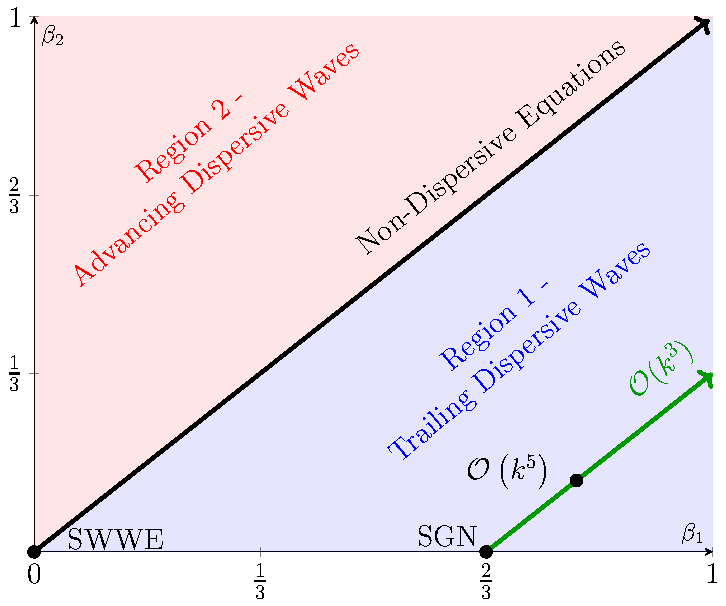
\includegraphics[width=0.4\textwidth]{./Figures/Explanation/BetaPlotAll.pdf}
	\caption{Phase speed regions of gSGN in terms of $\beta_1$ and $\beta_2$ showing important families of equations and particular members of these families.}
	\label{Fig:WaveSpeedReg}
\end{figure}


%-------------------------------------------------
\subsection{Alternative Conservative Form of the gSGN}
%-------------------------------------------------
\citet{Clamond-Dutykh-2018-237} demonstrate a rearrangement of \eqref{eq:gSGNuh} for the rSWWE, in an analogous way to the reformulations of SGN \cite{Hank-etal-2010-2034,Li-2014-169,Zoppou-etal-2017}. The purpose of this reformulation is to remove the mixed spatial-temporal derivative in the flux term, which is difficult to treat numerically. The reformulation works analogously for the gSGN equations as well, and thus an equivalent formulation of \eqref{eq:gSGNuh} can be obtained, giving
\begin{gather*}\label{eq:G_momentum}
\dfrac{\partial G }{\partial t}  + \dfrac{\partial}{\partial x} \left ( uG + \dfrac{gh^2}{2} - \left(\frac{2}{3} +  \beta_1\right) h^3\dfrac{\partial u}{\partial x}\dfrac{\partial u}{\partial x}  - \frac{1}{2} \beta_2 g h^2  \left[h\frac{\partial^2 h}{\partial x^2} + \frac{1}{2}\frac{\partial h}{\partial x}\frac{\partial h}{\partial x}\right]\right ) = 0
\end{gather*}
where the new conserved quantity
\begin{gather*}
G = hu - \frac{1}{2}\left(\frac{2}{3} + \beta_1\right) \dfrac{\partial }{\partial x} \left ( h^3 \dfrac{\partial u}{\partial x} \right ).
\end{gather*}
Using the appropriate substitution of $\beta_1$ values, the conserved variables introduced by \citet{Clamond-Dutykh-2018-237} for the rSWWE as well as for the SGN equations \cite{Hank-etal-2010-2034,Li-2014-169,Zoppou-etal-2017} can be obtained. 

Making this reformulation, provides the equation of mass for the gSGN and an equation in conservation law form for $G$ which is equivalent to the conservation of momentum equations as follows
\begin{subequations}
\begin{gather}
\dfrac{\partial h}{\partial t} + \dfrac{\partial (uh)}{\partial x} = 0
\label{eq:gSGN_Gh}
\end{gather}
\begin{gather}
\dfrac{\partial G }{\partial t}  + \dfrac{\partial}{\partial x} \left ( uG + \dfrac{gh^2}{2} - \frac{2}{3}\left(1 + \frac{3}{2} \beta_1\right) h^3\dfrac{\partial u}{\partial x}\dfrac{\partial u}{\partial x}  - \frac{1}{2} \beta_2 g h^2  \left[h\frac{\partial^2 h}{\partial x^2} + \frac{1}{2}\frac{\partial h}{\partial x}\frac{\partial h}{\partial x}\right]\right ) = 0.
\label{eq:gSGN_GG}
\end{gather}
with
\begin{gather}\label{eq:G_divergent}
G = uh - \frac{1}{3}\left(1 + \frac{3}{2} \beta_1\right) \dfrac{\partial }{\partial x} \left ( h^3 \dfrac{\partial u}{\partial x} \right ).
\end{gather}
\label{eq:gSGN_G}
\end{subequations}
This form of the equations and a bound on the wave speeds, allows \eqref{eq:gSGN_G} to be solved numerically using a combination of finite difference and finite volume methods as performed by \citet{Zoppou-etal-2017} for the SGN.

\section{Numerical Method}
The numerical method proposed for the gSGN, is very similar to methods published for the SGN \cite{Zoppou-etal-2017}. For brevity, only provide a general overview of the method is provided, with highlights of the important differences that need to be made to solve the gSGN instead of the SGN.

\subsection{Overview}
The numerical method for the gSGN equations proceeds very similarly to the SGN equations, space is discretised into cells of fixed width $\Delta x$, and time is partitioned into fixed time steps $\Delta t$. The midpoints of the $j^{th}$ cell are given by $x_j = x_0 + j \Delta x$, while the $n^{th}$ time step is given by $t^n = t^0 + n \Delta t$. Additionally for an arbitrary quantity $q$ the cell average of $q$ in the $j^{th}$ cell at time $t^n$ is defined as 
\[\bar{q}^n_j = \frac{1}{\Delta x} \int_{x_j - \Delta x / 2}^{x_j - \Delta x / 2} q(x,t^n) \; dx.\]
The overview will be using the value of quantities at all cells at a particular time and so $\vecn{q}^n$ is defined to be the vector of $q^n_j$ values and $\bar{\vecn{q}}^n$ to be the vector of $\bar{q}^n_j$ values for all cells in the domain. 

Following, \citet{Zoppou-etal-2017} the gSGN equations can be solved using the scheme outlined below beginning at a generic $n^{th}$ time step
\begin{enumerate}
	\item Begin with the vectors of cell averages $\bar{\vecn{h}}^n$ and $\bar{\vecn{G}}^n$.
	\item Solve \eqref{eq:G_divergent} with a second-order finite difference method using $\bar{\vecn{h}}^n$ and $\bar{\vecn{G}}^n$ to obtain an approximation to ${\vecn{u}}^n$, which can be written
	\[{A}\left(\bar{\vecn{h}}^n,\bar{\vecn{G}}^n\right) = {\vecn{u}}^n.\]
	\item Solve \eqref{eq:gSGN_Gh} and \eqref{eq:gSGN_GG} using a second-order finite volume method with the approximate Riemann solver of \citet{Kurganov-etal-2001-707} to obtain $\bar{h}^{n+1}_j$ and $\bar{G}^{n+1}_j$ at the next time step, obtaining
	\[{F}\left(\bar{\vecn{h}}^n,\bar{\vecn{G}}^n,{\vecn{u}}^n\right) = \bar{\vecn{h}}^{n+1 },\bar{\vecn{G}}^{n+1}.\]
	\item Combining these steps gives
	\[{E}(\bar{\vecn{h}}^{n},\bar{\vecn{G}}^{n}) = \bar{\vecn{h}}^{n+1 },\bar{\vecn{G}}^{n+1}.\]
	\item However, since ${F}$ is only first order accurate in time steps 1-4 are repeated and then fully second-order approximations to $\bar{\vecn{h}}^{n+1 }$,$\bar{\vecn{G}}^{n+1}$ are obtained using a SSP Runge Kutta method \cite{Gottlieb-etal-2003-89} like so
	\begin{align*}
	{E}(\bar{\vecn{h}}^{n},\bar{\vecn{G}}^{n}) &= \bar{\vecn{h}}^{'},\bar{\vecn{G}}^{'}\\
	{E}(\bar{\vecn{h}}^{'},\bar{\vecn{G}}^{'}) &= \bar{\vecn{h}}^{''},\bar{\vecn{G}}^{''}\\
	\frac{1}{2}\left(\bar{\vecn{h}}^{'} + \bar{\vecn{h}}^{''} \right) = \bar{\vecn{h}}^{n+1 } &\text{  and  }
		\frac{1}{2}\left(\bar{\vecn{G}}^{'} + \bar{\vecn{G}}^{''} \right) = \bar{\vecn{G}}^{n+1 }. 
	\end{align*}
\end{enumerate}

\subsection{Example Implementation}
Although the numerical method to solve the SGN demonstrated by \citet{Zoppou-etal-2017} can be readily adapted to the gSGN, there are some important differences. In particular, the reconstruction of $u$ must be modified to allow discontinuities, additional derivatives must be approximated and the wave speed bounds must be altered. 

\subsubsection{Reconstruction of $h$ and $G$}

\subsubsection{Reconstruction of $u$}

\subsubsection{Flux Approximation}

\subsubsection{Evolution Step}

\subsubsection{Runge-Kutta Time Stepping}



\section{Validation}
The numerical method described above is validated using analytic solutions for particular $\beta$ values that correspond to the SGN equations and the SWWE and a forced solution. Together these tests demonstrate the ability of the method to reproduce analytic solutions to important members of the gSGN family, as well as solve the gSGN for any pair of $\beta$ values that admit wave speed bounds.

The accuracy of the numerical method will be measured using the distance between the numerical solution and the equivalent analytic or forced solution using the $L_2$ norm. While the conservation properties of the numerical method will be measured by numerically approximating the energy in the initial conditions and the numerical solution and comparing them using a measure called $C_1$.

For a quantity $q$ with a vector of its analytic or forced solution at the cell midpoints $\vecn{q}$ and the numerical solution at the cell midpoints $\vecn{q}^*$, the discrete $L_2$ norm is
\begin{equation}
\label{eqn:Conv_Error}
L_2\left(\vecn{q},\vecn{q}^*\right) = \sqrt{ \dfrac{\sum_{j = 0}  \left[q_j^2 - \left(q^*_j\right)^2 \right]}{\sum_{j = 0}  \left[q_j^2 \right]}}
\end{equation}
where the time-step superscripts were suppressed for simplicity.

For a quantity $q$ with a vector of its values at the $n^{th}$ time step $\vecn{q}^n$, the total amount of the quantity is approximated by $C(\vecn{q}^n)$. The method for this is the same as the method described by \citet{Zoppou-etal-2017}, which has a higher order of accuracy than the numerical method it is measuring. Using the numerical approximation to the total amounts, the conservation error is obtained in the following way
\begin{equation}
\label{eqn:Cons_Error}
C_1\left(\vecn{q}^0,\vecn{q}^n\right) = \left \lbrace \begin{array}{l c r}
\dfrac{\left | C(\vecn{q}^0) - C(\vecn{q}^n) \right |}{\left| C(\vecn{q}^0) \right|}&,& \left| C(\vecn{q}^0) \right| > 0 \T \\
\left | C(\vecn{q}^0) - C(\vecn{q}^n) \right |&,& \left| C(\vecn{q}^0) \right| = 0 
\end{array} \right. .
\end{equation}

\begin{itemize}
	\item Analytic solutions - we recover them (conservation and norm)
	\item Forced solutions - our numerical method can handle any combination of beta values, all terms are approximated with correct order of accuracy. Limiters on gradients off. 
\end{itemize}

\subsection{Analytic Solutions}
The analytic solutions used to validate the numerical method, are the soliton solution of the SGN equations and the dam-break solution of the SWWE. The soliton solution is a smooth travelling wave solution, that assesses the balance of the non-linear and dispersive terms in the gSGN equations. Whereas the dam-break solution of the SWWE demonstrates the robustness of the method in the presence of steep gradients. The soliton solution used in this paper, is the same as the soliton solution used for validation by \citet{Pitt-2019}, allowing for a comparison of this gSGN solver to the more specialised SGN solvers described in that paper. 

\subsubsection{Serre Equations ($\beta_1=\beta_2 =0$) - Solitary Travelling Wave Solution}
When $\beta_1 = \beta_2 = 0$ the gSGN are equivalent to the SGN equations which admit the following travelling wave solution
\begin{subequations}
	\begin{equation}
	h(x,t) = a_0 + a_1 \text{sech}^2\left( \kappa (x - ct) \right),
	\end{equation}
	\begin{equation}
	u(x,t) = c \left( 1- \dfrac{a_0}{h(x,t)} \right),
	\end{equation}
	where
	\begin{equation}
	\kappa = \dfrac{\sqrt{3a_1}}{2a_0 \sqrt{a_0 + a_1}}
	\end{equation}
	and
	\begin{equation}
	c = \sqrt{g\left(a_0 + a_1\right)}.
	\end{equation}
\end{subequations}

This travelling wave solution is maintained due to a balance between the dispersive terms and the non-linear terms in the momentum equation \eqref{eq:G_momentum}. Validating the numerical solutions for the gSGN solver using this solution tests the balance between these terms in \eqref{eq:G_momentum}, and allows us to verify the method's conservation of energy as the solution is smooth. To enable a comparison between the numerical method and the SGN solver of \cite{Zoppou-etal-2017} the chosen soliton parameters were $a_0 = 1$ and $a_1 = 0.7$ and the acceleration due to gravity at the earth surface, $g = 9.81 m^2/s$ was used.

The numerical solution was solved over the domain $\left[-200,200\right]$ from $t=0s$ until $t=30s$. To ensure that the SGN solution is recovered, $\beta_1 = \beta_2=0$. The spatial resolution was varied like so $\Delta x = 400 / (100 \times 2^{l})$, where $l$ was increased. To satisfy the Courant-Friedrichs-Lewy (CFL) condition \cite{Lax-Richtmyer-1956-267} the time step width $\Delta t = \Delta x  / \left( 2 \sqrt{g \left(a_0 + a_1\right)}\right)$ \cite{Pitt-2019} was chosen. The limiting parameter $\theta$ was set to $\theta = 1.2$, matching the numerical experiments performed by \citet{Pitt-2019}.

Example numerical solutions for $h$, $u$ and $G$ with $\Delta x = 400 / (100 \times 2^{6}) \simeq 0.06m$ are plotted in Figure \ref{Fig:Sol_Ex}. These examples demonstrate that the numerical solutions well reproduced the analytic solutions.
%
\begin{figure}
	\centering
	\begin{subfigure}{0.32\textwidth}
		\centering
		\includegraphics[width=\textwidth]{./Figures/Simulations/Validation/Serre/h.pdf}
		\caption{$h$}
	\end{subfigure}
	\begin{subfigure}{0.32\textwidth}
		\centering
		\includegraphics[width=\textwidth]{./Figures/Simulations/Validation/Serre/G.pdf}
		\caption{$G$}
	\end{subfigure}
	\begin{subfigure}{0.32\textwidth}
		\centering
		\includegraphics[width=\textwidth]{./Figures/Simulations/Validation/Serre/u.pdf}
		\caption{$u$}
	\end{subfigure}
	\caption{Plot of comparing initial (\solidrule), analytic solution ({\color{blue}\solidrule}), and numerical solution with $\Delta x \approx 0.06m$ (\tikzcircle{red}) at $t = 30s$.}
	\label{Fig:Sol_Ex}
\end{figure}

A comparison of many numerical solutions with varying $\Delta x$ are given in Figure \ref{Fig:Sol_Comp} for both the convergence and conservation measures. These plots demonstrate that the scheme obtains second-order convergence for all quantities of interest, after $\Delta x$ becomes small enough to properly represent the initial conditions. 
%
\begin{figure}
	\centering
	\begin{subfigure}{0.49\textwidth}
		\centering
		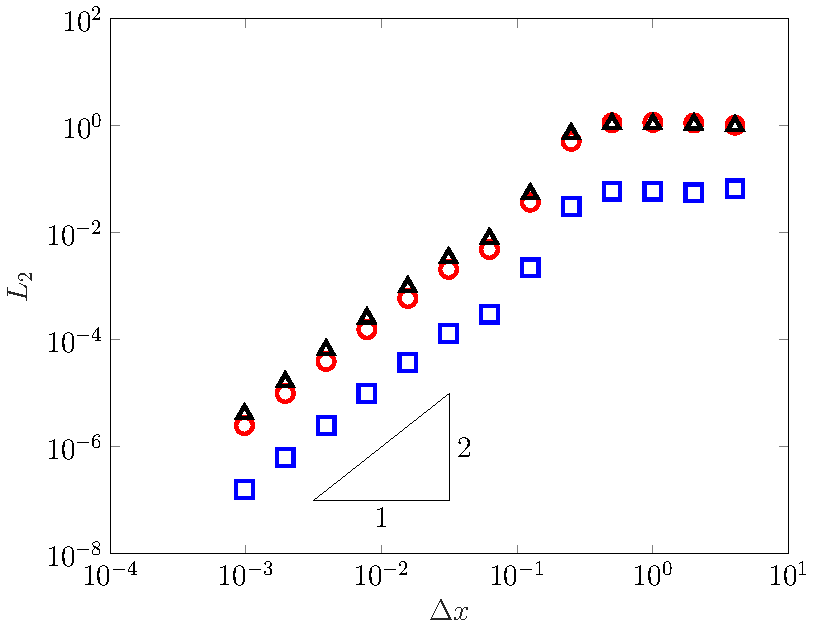
\includegraphics[width=\textwidth]{./Figures/Simulations/Validation/Serre/NormResults.pdf}
		\caption{$L_2$ with $u$ (\trianglet{black})}
		\label{Fig:Sol_Comp_Conv}
	\end{subfigure}
	\begin{subfigure}{0.49\textwidth}
		\centering
		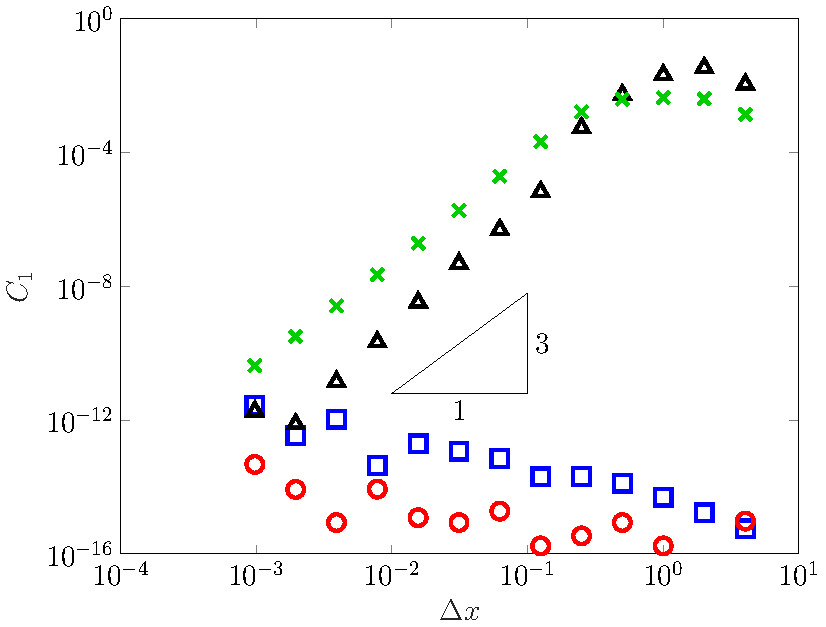
\includegraphics[width=\textwidth]{./Figures/Simulations/Validation/Serre/EnergyResults.pdf}
		\caption{$C_1$ with $uh$ (\trianglet{black})}
		\label{Fig:Sol_Comp_Cons}
	\end{subfigure}
	\caption{Convergence and conservation plots for $h$ (\squaret{blue}) , $G$ (\circlet{red}) and $\mathcal{H}$ (\crosst{green!60!black}) as $\Delta x$ varies.}
	\label{Fig:Sol_Comp}
\end{figure}
%
The conservation plot in Figure \ref{Fig:Sol_Comp_Conv} demonstrates that due to the use of the finite volume method $h$ and $G$ are conserved up to round-off error, which increases as $\Delta x$ increases. The conservation of $uh$ and $\mathcal{H}$ whilst not being at round-off error does reduce at a rate better than second-order and so the scheme possesses good convergence and conservation properties. These results agree well with the numerical solutions of \citet{Pitt-2019}, who compared various numerical methods. 

\subsubsection{SWWE ( $\beta_1= -\frac{2}{3}$ and $ \beta_2 =0$ ) - Dam-break Solution }
When $\beta_1= -\frac{2}{3}$ and $ \beta_2 =0$ the gSGN equations reduce to the SWWE which have an analytic solution to the dam-break problem given by the initial conditions
\begin{align}
h(x,0) & = \left\lbrace \begin{array}{c c}
h_0 & x < 0\\
h_1 & x \ge 0
\end{array} \right.  \\
u(x,0) &= 0 \\
G(x,0) &= 0.
\end{align}

The solution to the dam-break problem is given by
\begin{align}
h(x,t) &= \left \lbrace \begin{array}{l c r}
h_0 &,& x \le -t\sqrt{g h_0} \\
\frac{4}{9g} \left(\sqrt{gh_0} - \frac{x}{2t}\right)^2 &,&  -t\sqrt{g h_0} < x \le t \left(u_2 - \sqrt{g h_2}\right)  \\
h_2 &,&  t \left(u_2 - \sqrt{g h_2}\right) < x \le t S_2  \\
h_1 &,&   t S_2 \le x \\
\end{array} \right.  \\
u(x,t) &= \left \lbrace \begin{array}{l c r}
0 &,& x \le -t\sqrt{g h_0} \\
\frac{2}{3} \left(\sqrt{gh_0} + \frac{x}{t}\right) &,&  -t\sqrt{g h_0} < x \le t \left(u_2 - \sqrt{g h_2}\right)  \\
u_2 &,&  t \left(u_2 - \sqrt{g h_2}\right) < x \le t S_2  \\
0 &,&   t S_2 \le x \\
\end{array} \right. .
\end{align}
%
The constant state values $h_2$ and $u_2$ and the shock speed $S_2$ can be calculated for any initial conditions by solving
\begin{align}
\label{eq:SWWEMiddleState}
h_2 &= \dfrac{h_0}{2} \left(  \sqrt{1 + 8 \left( \dfrac{2 h_2}{h_2 - h_0} \left(\dfrac{\sqrt{gh_1} - \sqrt{gh_2}}{\sqrt{gh_0}}\right)\right)^2 } - 1 \right) \\
u_2 &= 2\left(\sqrt{gh_1} - \sqrt{gh_2} \right),\\
S_2 &= \dfrac{2 h_2}{h_2 - h_1}\left(\sqrt{gh_0} - \sqrt{gh_2} \right).
\end{align}

The initial conditions as well as the analytic solution are discontinuous. Due to the discontinuities the solutions to the initial conditions are not unique, as solving any pair of the 3 conservation equations \eqref{eq:gSGN}, gives solutions with similar structures but different constant values. The solution presented above is solution of the mass and momentum equations, as these equations are the basis of the numerical method.

A number of numerical experiments were run for the dam-break problem with $h_0 = 2m$ and $h_1 = 1m$. The domain of the solution was $\left[-250,250\right]$ with a final time of $t=35s$.  The spatial resolution was varied like so $\Delta x = 500 / (1000 \times 2^{l})$, while to satisfy the CFL condition \cite{Lax-Richtmyer-1956-267} the time step width $\Delta t = \Delta x  / \left( 2 \sqrt{g h_0}\right)$ was used. The limiting parameter $\theta$ was set to be $\theta = 1.2$ and the acceleration due to gravity $g = 9.81 m^2/s$ was used. 

Example numerical solutions and analytic solutions for $h$, $G$ and $u$ at the final time with the spatial resolution $\Delta x = 500 / (1000 \times 2^{4})$ are plotted in Figure \ref{Fig:DB_Ex}. These figures demonstrate that the method is robust in the presence of steep gradients and appropriately reproduces the broad structure of the analytic solution. 
%
\begin{figure}
	\centering
	\begin{subfigure}{0.32\textwidth}
		\centering
		\includegraphics[width=\textwidth]{./Figures/Simulations/Validation/DBSWWE/h.pdf}
		\caption{$h$}
	\end{subfigure}
	\begin{subfigure}{0.32\textwidth}
		\centering
		\includegraphics[width=\textwidth]{./Figures/Simulations/Validation/DBSWWE/G.pdf}
		\caption{$G = uh$}
	\end{subfigure}
	\begin{subfigure}{0.32\textwidth}
		\centering
		\includegraphics[width=\textwidth]{./Figures/Simulations/Validation/DBSWWE/u.pdf}
		\caption{$u$}
	\end{subfigure}
	\caption{Comparison of initial (\solidrule), analytic solution ({\color{blue}\solidrule}), and numerical solution with $\Delta x \approx 0.03m$ (\tikzcircle{red}) at  $t=35s$.}
	\label{Fig:DB_Ex}
\end{figure}

The central difficulty of reproducing the analytic solutions for the dam-break problem, is observed around only a few critical locations; the top of the rarefaction fan, the bottom of the rarefaction fan and the shock front. Figure \ref{Fig:Conv_Ex} demonstrates the convergence of the solutions for $h$ as $\Delta x$ changes for the top of the rarefaction fan and the shock front. 
%
\begin{figure}
	\centering
	\begin{subfigure}{0.45\textwidth}
		\centering
		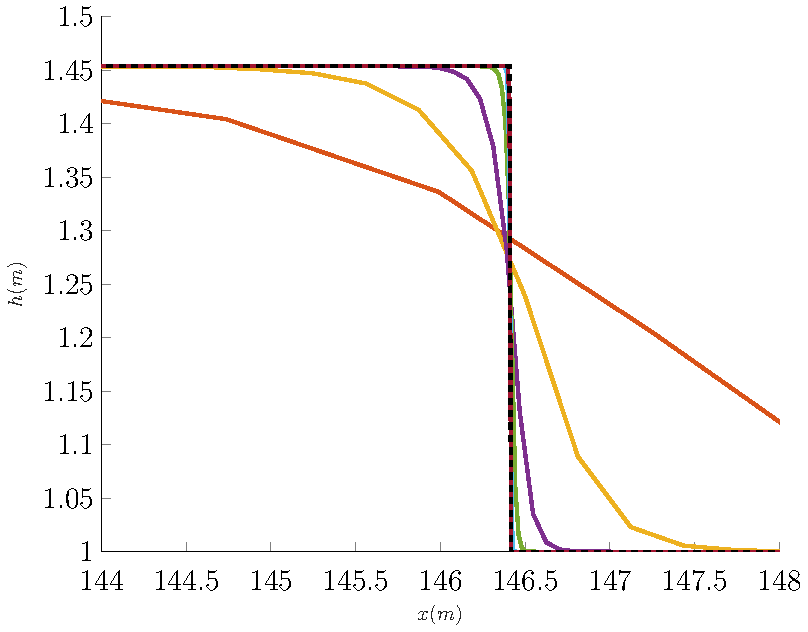
\includegraphics[width=\textwidth]{./Figures/Simulations/Validation/DBSWWE/hFront.pdf}
		\caption{Shock front}
	\end{subfigure}
	\begin{subfigure}{0.45\textwidth}
		\centering
		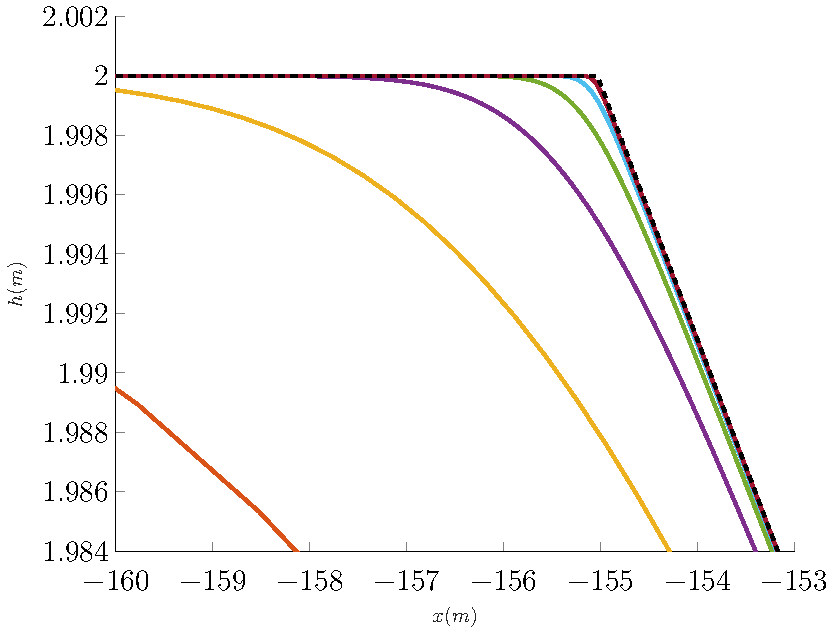
\includegraphics[width=\textwidth]{./Figures/Simulations/Validation/DBSWWE/hRFTop.pdf}
		\caption{Top of rarefaction fan}
	\end{subfigure}
	\caption{Plots of $h$ at $t=35s$ for the smooth dam-break problem around important locations with $\Delta x = 2^{-1}$ ({\color{mycolor1}\solidrule}), $2^{-2}$ ({\color{mycolor2}\solidrule}), $2^{-3}$ ({\color{mycolor3}\solidrule}), $2^{-4}$ ({\color{mycolor4}\solidrule}), $2^{-5}$ ({\color{mycolor5}\solidrule}), $2^{-6}$ ({\color{mycolor6}\solidrule}), $2^{-7}$ ({\color{mycolor7}\solidrule}), $2^{-8}$ ({\color{mycolor1}\solidrule}) and the analytic solution ({\dashedrule}) of the SWWE to the corresponding dam-break problem.}
	\label{Fig:Conv_Ex}
\end{figure}
%
Figure \ref{Fig:Conv_Ex} demonstrates that as $\Delta x$ decreases tje numerical solutions are converging to better resolve these critical locations. The behaviour of the bottom of the rarefaction fan is very similar to the top, and the behaviour of the solutions for $u$ and $G$ is similar, and so has been omitted. The convergence of the numerical methods is difficult to measure since the solutions are discontinuous, and so this more visual approach is used. In the presence of discontinuities the method is no longer expected to be fully second-order accurate, due to the use of the limiters, even so the method still possesses good convergence properties in the presence of the discontinuities.

Figure \ref{Fig:DB_Cons} shows the conservation properties of the numerical solutions as $\Delta x$ decreases. The conservation of $h$ and $G=uh$ is at round-off error and thus the error gets larger as $\Delta x$ decreases and the number of calculations increases. The conservation of $u$ is now only first-order, while the conservation of $\mathcal{E}$ doesn't improve as $\Delta x$ decreases. The drop in order for conservation of $u$ is due to the use of limiters which whilst making the numerical method total variation diminishing \cite{LeVeque-2002} and more robust, also result in the reconstruction becoming first-order near discontinuities. The lack of improvement in conservation of $\mathcal{E}$ is because the solutions are not sufficiently smooth, and thus do not satisfy all conservation equations \eqref{eq:gSGN} simultaneously \cite{Pu-2018-1361}. The loss of conservation in $\mathcal{H}$ is also a feature of the analytic solution as can be seen in Figure \ref{Fig:DB_Energy} which plots the total amount of energy over time for numerical and the analytic solutions. 
%
%Remove uh and energy, since energy dissipated anyway
\begin{figure}
	\centering
	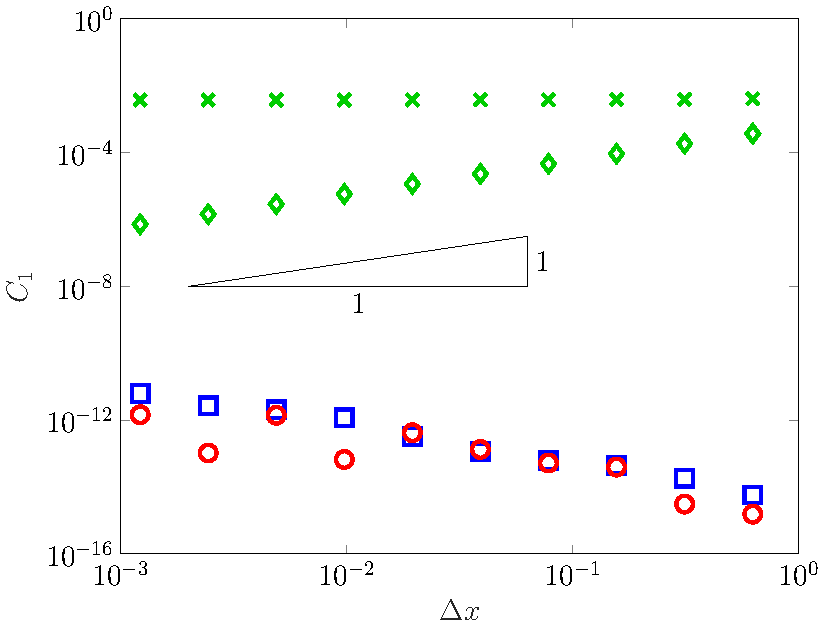
\includegraphics[width=0.5\textwidth]{./Figures/Simulations/Validation/DBSWWE/EnergyResults.pdf}
	\caption{Conservation Plots  $h$ (\squaret{blue}) , $G$ (\circlet{red}), $uh$ (\trianglet{black}), $\mathcal{H}$ \crosst{green!60!black}.}
	\label{Fig:DB_Cons}
\end{figure}
%
\begin{figure}
	\centering
	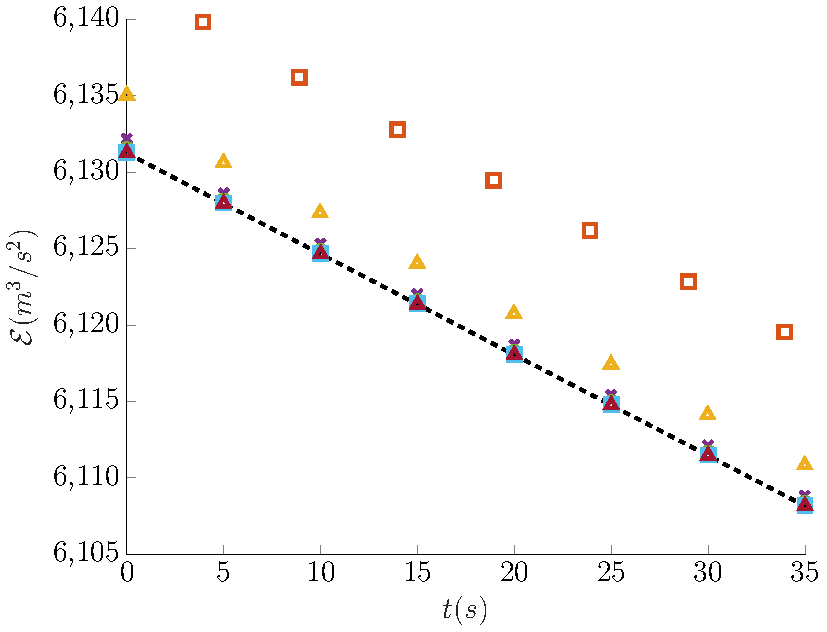
\includegraphics[width=0.49\textwidth]{./Figures/Simulations/Validation/DBSWWE/EnergyOverTime.pdf}
	\caption{Plot of total energy $\mathcal{H}$ for numerical solutions over time with $\Delta x = 2^{-1}$ ({\color{mycolor1}\circlet{}}), $2^{-2}$ ({\color{mycolor2}\squaret{}}), $2^{-3}$ ({\color{mycolor3}\trianglet{}}), $2^{-4}$ ({\color{mycolor4}\crosst{}}), $2^{-5}$ ({\color{mycolor5}\circlet{}}), $2^{-6}$ ({\color{mycolor6}\squaret{}}), $2^{-7}$ ({\color{mycolor7}\trianglet{}}), $2^{-8}$ ({\color{mycolor1}\crosst{}}) and the analytic solution ({\solidrule}) of the SWWE to the corresponding dam-break problem..}
	\label{Fig:DB_Energy}
\end{figure}

These results demonstrate that the analytic solution of the SWWE has been accurately reproduced by the numerical method. 

\subsection{Forced Solutions}
To demonstrate the validity and versatility of the method to solve the gSGN for any $\beta$ values, forced solutions were used. To generate a forced solution the forced gSGN equations are considered
\begin{subequations}
	\begin{gather}
	\dfrac{\partial h}{\partial t} + \dfrac{\partial (uh)}{\partial x} = \dfrac{\partial h^*}{\partial t} + \dfrac{\partial (u^*h^*)}{\partial x} 
	\label{eq:gSGN_Gh_Forced}
	\end{gather}
	\begin{multline}
	\dfrac{\partial G }{\partial t}  + \dfrac{\partial}{\partial x} \left ( uG + \dfrac{gh^2}{2} - \frac{2}{3}\left(1 + \frac{3}{2} \beta_1\right) h^3\dfrac{\partial u}{\partial x}\dfrac{\partial u}{\partial x}  - \frac{1}{2} \beta_2 g h^2  \left[h\frac{\partial^2 h}{\partial x^2} + \frac{1}{2}\frac{\partial h}{\partial x}\frac{\partial h}{\partial x}\right]\right ) = \\ \dfrac{\partial G^* }{\partial t}  + \dfrac{\partial}{\partial x} \left ( u^*G^* + \dfrac{g\left(h^*\right)^2}{2} - \frac{2}{3}\left(1 + \frac{3}{2} \beta_1\right) \left(h^*\right)^3\dfrac{\partial u^*}{\partial x}\dfrac{\partial u^*}{\partial x}  - \frac{1}{2} \beta_2 g \left(h^*\right)^2  \left[h^*\frac{\partial^2 h^*}{\partial x^2} + \frac{1}{2}\frac{\partial h^*}{\partial x}\frac{\partial h^*}{\partial x}\right]\right ).
	\label{eq:gSGN_GG_Forced}
	\end{multline}
	\label{eq:gSGN_Forced}
\end{subequations}
The forced gSGN admit the solutions $h^*$, $u^*$ and $G^*$ assuming $G^*$ appropriately satisfies \eqref{eq:G_divergent}. Since these equations are satisfied for any chosen $h^*$, $u^*$ and $G^*$ and any $\beta$ values, forced solutions can be used to verify the method for a large class of problems. Since the left hand-side of these modified equations are approximated by the numerical method, by combining the numerical method with the analytic expressions for the right hand-side, produces a method that approximates the forced gSGN equation with the same convergence properties as the underlying numerical method for the gSGN equations. 

Since $h^*$, $u^*$ and $G^*$ are arbitrary any desires solution can be generated and used to test the convergence properties for situations for which no known analytic solution to the equations exist. Of particular in this paper are solutions where the $\beta$ values are not equivalent to well studied equations and thus have no known analytic solutions exist, and where all the terms in the equations are non-zero, and thus must be approximated accurately. 

To accomplish these goals the following forced solutions
\begin{subequations}
	\begin{equation}
	h^*(x,t) = a_0 + a_1 \exp\left( \dfrac{\left(x - a_2 t\right)^2}{2 a_3} \right)
	\end{equation}
	\begin{equation}
	u^*(x,t) = a_4 \exp\left( \dfrac{\left(x - a_2 t\right)^2}{2 a_3} \right)
	\end{equation}
	\begin{align}
	\beta_1(x,t) &= a_6 \\
	\beta_2(x,t) &= a_7
	\end{align}
\end{subequations}
where $G^*$ is given by \eqref{eq:G_divergent}, were used. These forced solutions describe Gaussian bumps in $h$ and $u$ that travel at a constant speed $a_2$. The particular parameter values $a_0=1$, $a_1=0.5$, $a_3=20$, $a_4=0.3$, $a_6 = 1$ and $a_7=2$ were chosen in this investigation. Note that using these values, all terms in \eqref{eq:gSGN_G} are non-zero, and thus must be accurately approximated by the numerical method to reproduce the forced solution.

The numerical solutions were produced over the domain $\left[-100,100\right]$ with a final time of $t=10$. The spatial resolution was varied like so $\Delta x = 200 / (100 \times 2^{l})$, while the CFL condition was satisfied by setting $\Delta t = \Delta x  / \left( 2 \left[a_4 + a_2+ \sqrt{g \left(a_0 + a_1\right)}\right] \right)$. The acceleration due to gravity $g=9.81m^2/s$ and the limiting parameter $\theta = 1.2$ was used.

Figure \ref{Fig:FS_Ex} shows example numerical solutions at the final time for $h$, $G$ and $u$ with $\Delta x = 200 / (100 \times 2^{6}) \approx 0.03$. These example solutions demonstrate that the numerical method is able to reproduce the forced solution well.
%
\begin{figure}
	\centering
	\begin{subfigure}{0.32\textwidth}
		\centering
		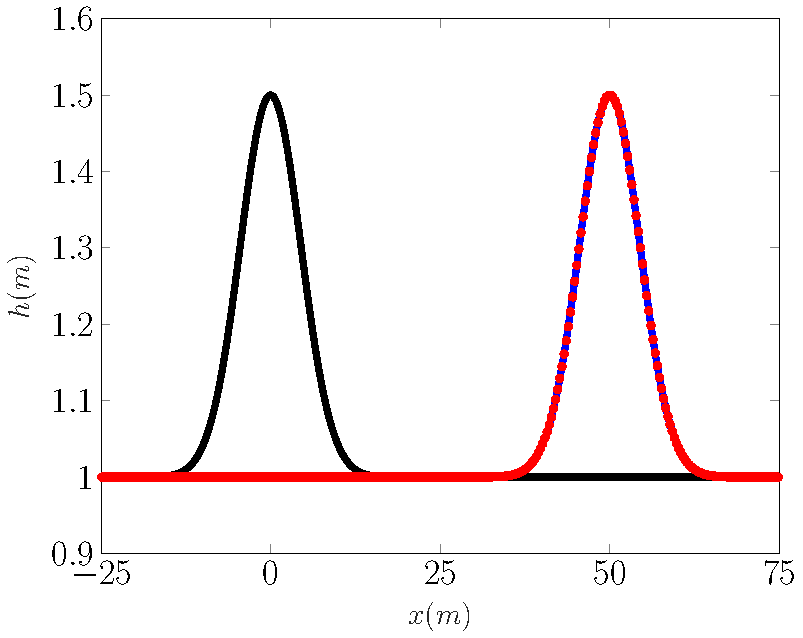
\includegraphics[width=\textwidth]{./Figures/Simulations/Validation/Forced/h.pdf}
		\caption{$h$}
	\end{subfigure}
	\begin{subfigure}{0.32\textwidth}
		\centering
		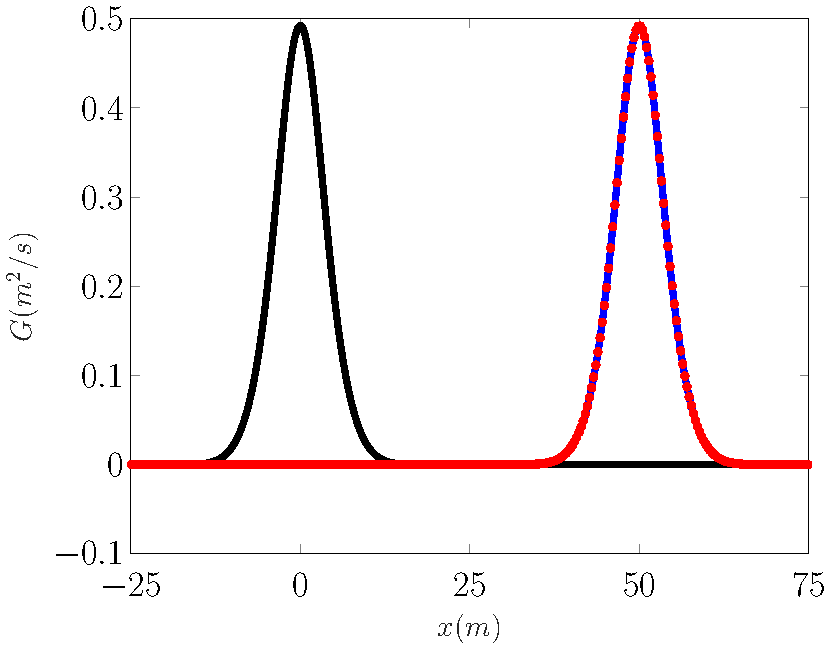
\includegraphics[width=\textwidth]{./Figures/Simulations/Validation/Forced/G.pdf}
		\caption{$G$}
	\end{subfigure}
	\begin{subfigure}{0.32\textwidth}
		\centering
		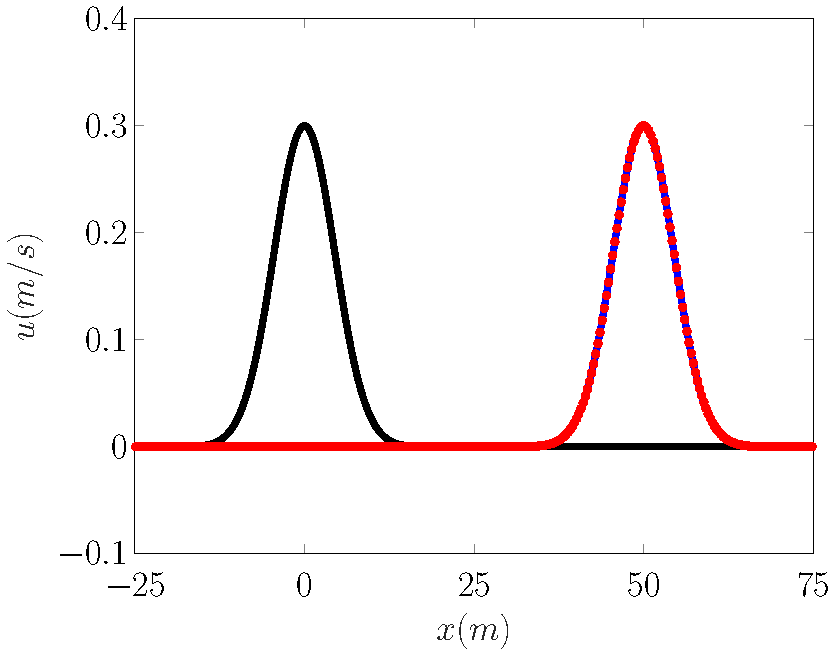
\includegraphics[width=\textwidth]{./Figures/Simulations/Validation/Forced/u.pdf}
		\caption{$u$}
	\end{subfigure}
	\caption{Example plots Initial (\solidrule), analytic solution ({\color{blue}\solidrule}), and numerical solution with $\Delta x \approx 0.03m$ (\tikzcircle{red}).}
	\label{Fig:FS_Ex}
\end{figure}

Figure \ref{Fig:FS_Conv} demonstrates the convergence of the numerical scheme as $\Delta x$ decreases. All quantities of interest are converging at the expected second-order. Since the RHS is given analytically, the observed error is caused by the numerical method. Therefore, these results demonstrate that the scheme is second-order for all terms in gSGN equations. Unfortunately, to be able to accurately reproduce the forced solutions the limiting on the derivatives had to be removed. This made the derivative approximations consistent, and importantly didn't restrict the derivatives at the top of the Gaussian bumps. Thus the forced solutions only validate the method without derivative limiting for all $\beta$ values. However, given that the limiting is only comparing derivative approximations of the same order and the above analytic solutions, the numerical method is well validated.
%
\begin{figure}
	\centering
	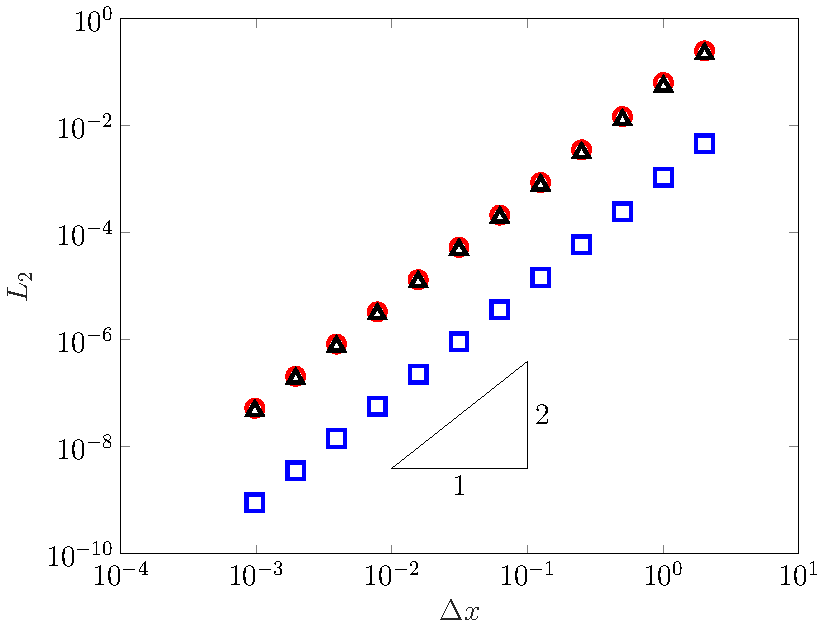
\includegraphics[width=0.49\textwidth]{./Figures/Simulations/Validation/Forced/NormResults.pdf}
	\caption{Convergence plot of $h$ (\squaret{blue}) , $G$ (\circlet{red}), $u$ (\trianglet{black}) for the forced solutions for various $\Delta x$ values.}
	\label{Fig:FS_Conv}
\end{figure}


\section{Conclusion}
A modified version of the SGN solver outlined by \citet{Zoppou-etal-2017} was used to solved the gSGN equations which make the constant in front of the dispersive term free and adds a surface tension-like regularisation term \cite{Clamond-et.al-2017-245,Clamond-Dutykh-2018-237}. The new gSGN solver was validated against analytic solutions of the SGN and SWWE equations and forced solutions. The analytic solutions demonstrate that the gSGN solver accurately reproduces important members of the gSGN family of equations whilst conserving the quantities of interest for sufficiently smooth solutions, and the forced solutions demonstrate that the method remains second-order for all values of the free parameters, $\beta_1$ and $\beta_2$. The gSGN method described above is the first well validated numerical method for the gSGN equations and the rSWWE and iSGN families of equations. The numerical method is then used to verify and expand numerical results in the literature for the smoothed dam-break problem \cite{Clamond-Dutykh-2018-237,Clamond-et.al-2017-245,Pu-2018-1361}. The first set of these experiments demonstrate the rSWWE family possesses regularised numerical solutions that converge nicely as the SWWE are approached. Additionally, the numerical results for energy dissipation agree with the analytic result of \citet{Pu-2018-1361}, where the weak singularities associated with this dissipation can be seen in plots of the conserved quantity $G$. The second group of experiments demonstrate the behaviour of the iSGN family of equations, which agrees very well with the linear theory. The results demonstrate that for steep gradient problems the iSGN family will require higher resolution grids or higher order methods to resolve the dispersive wave train around the high wave-number limits. Finally, the numerical solutions for the family of equations that lie between the SGN and SWWE equations, the SGN to SWWE family were studied. These results demonstrate that even for very small $\beta_1$ values steep gradients will develop extensive dispersive wave trains and when $\beta_1$ is close to the critical SWWE value, then the solutions of the SGN to SWWE family dissipate energy at the same rate as the SWWE for the numerical solutions. 

\bibliographystyle{unsrtnat}
\bibliography{Bibliography}


\end{document} 